\documentclass{beamer}
\usetheme{Madrid}
\usecolortheme{default}
\usepackage{graphicx}
\usepackage{booktabs}
\usepackage{listings}
\usepackage{xcolor}
\setbeamertemplate{navigation symbols}{}
\setbeamertemplate{caption}[numbered]

\definecolor{codebg}{RGB}{245,245,245}
\definecolor{codekw}{RGB}{0,90,140}
\definecolor{codecom}{RGB}{110,110,110}
\definecolor{codestr}{RGB}{160,40,40}
\lstdefinestyle{py}{
    backgroundcolor=\color{codebg},
    basicstyle=\ttfamily\scriptsize,
    keywordstyle=\color{codekw}\bfseries,
    commentstyle=\color{codecom}\itshape,
    stringstyle=\color{codestr},
    language=Python,
    showstringspaces=false,
    frame=single,
    rulecolor=\color{gray},
    numbers=none,
    breaklines=true,
    tabsize=2,
}
\lstdefinestyle{term}{
    backgroundcolor=\color{black},
    basicstyle=\ttfamily\scriptsize\color{green!70!black},
    frame=single,
    breaklines=true,
}

\title{ByteNet: Rethinking Multimedia File Fragment Classification Through Visual Perspectives}
\subtitle{A Reproduction Study -- Implementation, Training \& Results}
\author{Payaldurga Paila \and Mehul \and Arpita}
\institute{Indian Institute of Information Technology Vadodara \\ \small{Under the guidance of Prof. Jignesh Patel}}
\date{}

\begin{document}

% ------------------------------------------------------
\begin{frame}
    \titlepage
\end{frame}

% ------------------------------------------------------
\begin{frame}{Problem Definition}
A fragment is a fixed-size chunk of a file -- 512 bytes off a disk sector,
say, or out of a network packet -- with no filename, no extension, and
nothing attached to say what kind of file it came from.

Guessing the file type from that chunk alone is what file fragment
classification tries to do, and it's harder than it sounds:
\begin{itemize}
    \item a fragment can come from anywhere in a file, not just the start,
    so a magic-byte signature like \texttt{FFD8} for JPEG isn't guaranteed
    to even be present
    \item most prior learning-based methods -- Byte2Vec, FiFTy, DSCNN --
    read a fragment as a flat 1D sequence, so they only ever compare a
    byte to \emph{other separate bytes} (interbyte relationships)
\end{itemize}
In practice this comes up in digital forensics, pulling files off damaged
storage, and in network security, inspecting traffic where headers have
been stripped or corrupted.
\end{frame}

% ------------------------------------------------------
\begin{frame}{Why Interbyte-Only Methods Fall Short}
Byte2Image is built around a specific gap in the sequence-only view: a
byte has 8 bits, and nothing forces the patterns worth learning to line
up neatly with byte boundaries.

JPEG is the clean example. Its DCT coefficients are Huffman coded, and
Huffman codes are variable-length -- a single symbol (the paper uses the
pair ``(4)'' and ``(-9)'' in its own Fig.~3) can start in the middle of
one byte and finish in the middle of the next. A model that only ever
compares byte $N$ to byte $N{+}1$ has no way to see that pattern, because
the pattern doesn't respect byte boundaries at all.

\vspace{0.5em}
The fix is almost mechanical: bit-shift the fragment seven times and
stack the results, and the bits inside a byte become just as visible to
the model as the bytes themselves.
\end{frame}

% ------------------------------------------------------
\begin{frame}{Byte2Image: The Transform}
Turning a byte fragment into an image happens in three steps, each one
addressing a problem the step before it leaves behind:

\begin{enumerate}
    \item \textbf{Bit-shift.} Given a fragment of $N_s$ bytes, compute
    $x_0 = x$ and $x_i = (x_{i-1} \ll 1) \bmod 256$ for $i = 1, \dots, 7$.
    Stacking these seven shifted copies row-wise gives a matrix
    $x_{\text{in}} \in \mathbb{Z}^{N_s \times 8}$: each \emph{row} carries
    intrabyte (bit-level) structure, each \emph{column} keeps the
    original interbyte structure intact.
    \item \textbf{Intrabyte n-gram.} $x_{\text{in}}$ is only 8 pixels
    wide, which convolutional layers handle badly. Grouping $n$
    consecutive rows and concatenating them column-wise produces a
    near-square image of shape $(N_s - n + 1,\ 8n)$ instead.
    \item \textbf{Augment.} Horizontal flip, random erase, and mixup --
    standard moves, needed here because the fragment count itself can't
    grow.
\end{enumerate}
\end{frame}

% ------------------------------------------------------
\begin{frame}{Byte2Image in Action -- Real Output}
Nothing here is a mockup -- this came straight out of running our own
\texttt{bytenet/byte2image.py} on a real 256-byte PNG fragment pulled
from the dataset:
\begin{center}
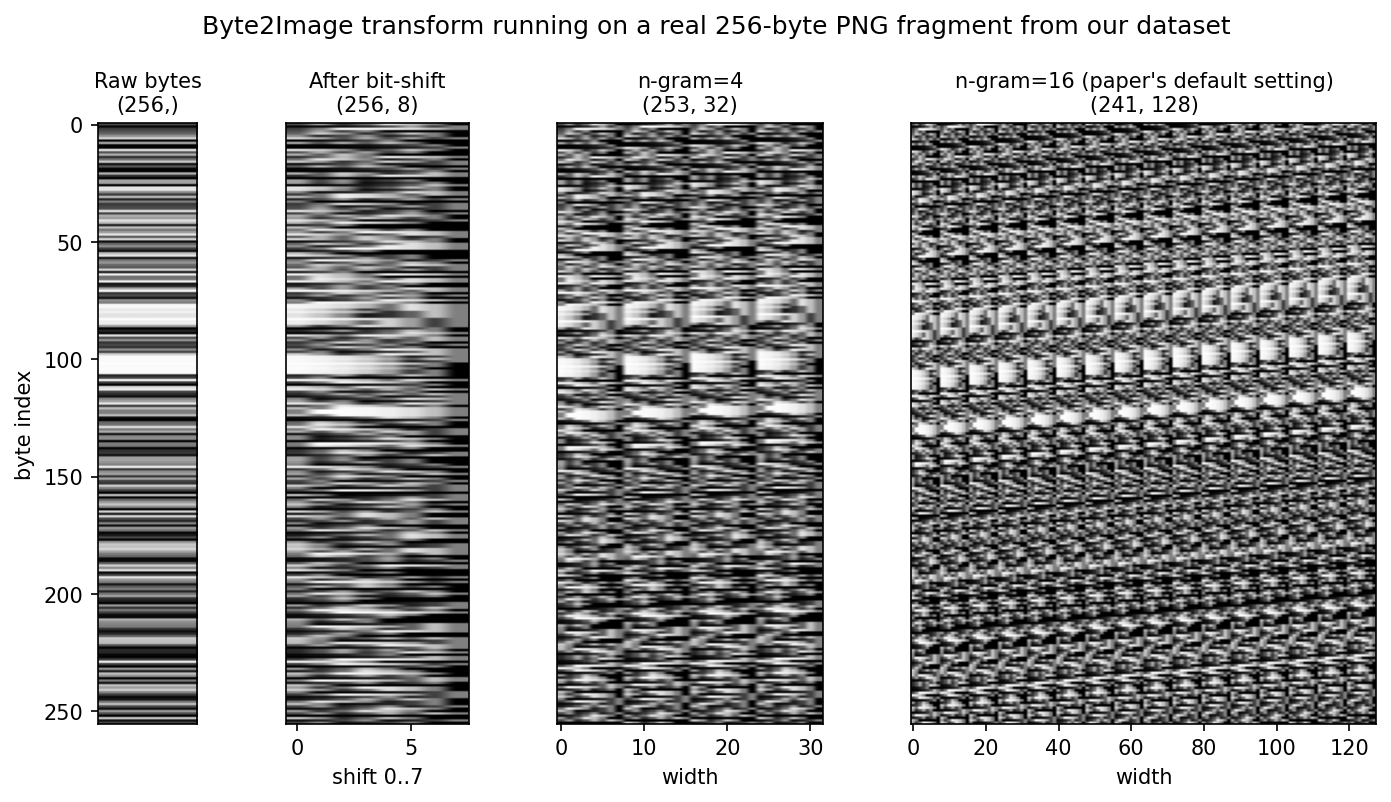
\includegraphics[width=0.92\linewidth]{figures/byte2image_demo.png}
\end{center}
{\footnotesize Left to right: the raw byte column, the $(256,8)$ matrix
after bit-shifting, the n-gram=4 image we trained on, and n-gram=16 --
the paper's default setting. The n-gram step is the one doing visible
work: the image goes from a thin strip to something with real structure.}
\end{frame}

% ------------------------------------------------------
\begin{frame}[fragile]{Code: The Bit-Shift Step}
This is the core of Byte2Image as it sits in
\texttt{bytenet/byte2image.py}:
\begin{lstlisting}[style=py]
def bit_shift_stack(byte_seq: np.ndarray) -> np.ndarray:
    """Eq. (2): x0 = x, xi = (x_{i-1} << 1) mod 256."""
    byte_seq = np.asarray(byte_seq, dtype=np.uint8)
    ns = byte_seq.shape[0]
    x_in = np.empty((ns, 8), dtype=np.uint8)
    cur = byte_seq.copy()
    for i in range(8):
        x_in[:, i] = cur
        cur = ((cur.astype(np.uint16) << 1) & 0xFF).astype(np.uint8)
    return x_in
\end{lstlisting}
It's a near-literal reading of the paper's Eq.~(2) -- each output column
is the fragment shifted one bit further left than the column before it.
\end{frame}

% ------------------------------------------------------
\begin{frame}{ByteNet Architecture}
\begin{center}
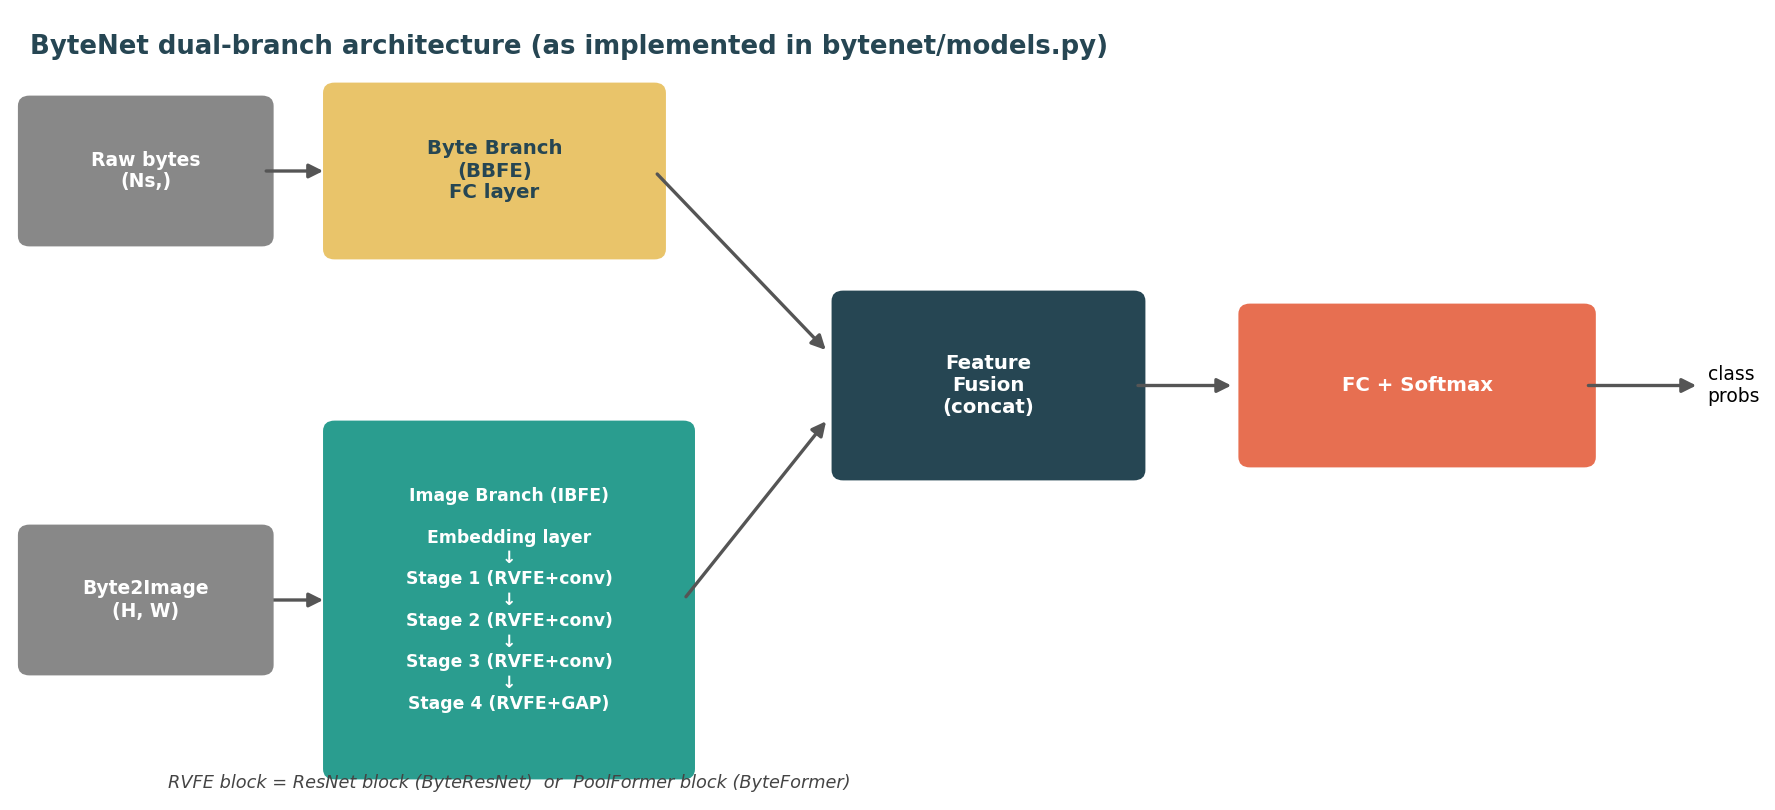
\includegraphics[width=0.82\linewidth]{figures/architecture_diagram.png}
\end{center}
\small
The byte branch is deliberately small -- one fully-connected layer over
the raw bytes, mainly there to catch magic-byte co-occurrences like
\texttt{FFD8} for JPEG. The image branch does the heavy lifting: an
embedding layer feeds four stages of residual blocks, each one
downsampling before the next, ending in a global average pool.
Concatenate what comes out of both branches, run it through one more
linear layer with softmax, and that's the whole classifier.
\end{frame}

% ------------------------------------------------------
\begin{frame}[fragile]{Code: Dual-Branch Fusion}
And here's that fusion step for real, straight out of the
\texttt{forward()} method of our \texttt{ByteNet} class in
\texttt{bytenet/models.py}:
\begin{lstlisting}[style=py]
def forward(self, raw_bytes, img):
    # raw_bytes: (B, Ns) in [0,1]; img: (B, 1, H, W) in [0,1]
    x_sf = self.byte_branch(raw_bytes)

    x = self.embed(img)
    for stage in self.stages:
        x = stage(x)
    x_df = x.flatten(1)  # after GAP: (B, C4, 1, 1) -> (B, C4)

    fused = torch.cat([x_sf, x_df], dim=1)
    logits = self.classifier(fused)
    return logits
\end{lstlisting}
\texttt{x\_sf} is what the byte branch produces, \texttt{x\_df} is the
image branch's output after its last global average pool -- concatenating
them is literally the fusion box in the diagram, nothing more exotic.
\end{frame}

% ------------------------------------------------------
\begin{frame}{Two Variants: ByteResNet vs. ByteFormer}
The image branch can be built from two different block types, which is
where the paper's two named variants come from -- both live in our
\texttt{RVFEStage} class:

\begin{columns}
\column{0.48\textwidth}
\textbf{ByteResNet}
\begin{itemize}
    \item wide n-gram embedding convolution
    \item classic \texttt{ResNetBlock}: two $3\times3$ convs, batch norm,
    residual connection
    \item 489K parameters
\end{itemize}
\column{0.48\textwidth}
\textbf{ByteFormer}
\begin{itemize}
    \item patch embedding, splits the image into patches
    \item \texttt{PoolFormerBlock}: a pooling-based token mixer plus a
    channel MLP, no attention involved
    \item 186K parameters, and roughly 15$\times$ faster per epoch on CPU
\end{itemize}
\end{columns}
\vspace{0.6em}
We trained both, end to end, to see how they actually compare rather than
take the paper's word for it.
\end{frame}

% ------------------------------------------------------
\begin{frame}{Building a Real Dataset}
FFT-75 and VFF-16, the benchmarks the paper actually trains on, weren't
reachable from where we were building this. Rather than feed the network
random noise and call it a test, we pointed
\texttt{bytenet/data\_prep.py} at the local filesystem instead: seven
file types, and for each one, 256-byte windows cut from random offsets
inside real files -- \texttt{.py}, \texttt{.json}, \texttt{.html},
\texttt{.png}, \texttt{.pdf}, \texttt{.gz}, and ELF binaries. That's
close to how FFT-75 itself was assembled, just from GovDocs documents
instead of whatever happened to be sitting on this machine.

\begin{itemize}
    \item 320 fragments per class, 2{,}240 total
    \item 80/20 train/test split
\end{itemize}
Because the offsets are random, a fragment landing on a file's header is
mostly luck -- the model can't lean on magic bytes being there.
\end{frame}

% ------------------------------------------------------
\begin{frame}[fragile]{Dataset Build -- Real Console Output}
What actually printed when we ran the builder:
\begin{lstlisting}[style=term]
$ python -m bytenet.data_prep --sector-size 256 --per-class 320
Saved 2240 sectors of size 256 bytes -> data/fragments.npz
Classes: ['elf', 'gz', 'html', 'json', 'pdf', 'png', 'py']
  elf   :  320 sectors from 2637 files
  gz    :  320 sectors from 1376 files
  html  :  320 sectors from  398 files
  json  :  320 sectors from 1470 files
  pdf   :  320 sectors from  804 files
  png   :  320 sectors from  551 files
  py    :  320 sectors from 4000 files
\end{lstlisting}
Every class draws its 320 fragments from hundreds to thousands of
distinct source files -- no single file is carrying an entire class.
\end{frame}

% ------------------------------------------------------
\begin{frame}{Training Setup}
We stuck to the paper's training recipe (Sec.~IV-B) as closely as a
single CPU core allows:

\begin{center}
\begin{tabular}{ll}
\toprule
\textbf{Setting} & \textbf{Value} \\
\midrule
Optimizer & AdamW, weight decay 0.01 \\
LR schedule & Cosine decay, linear warmup \\
Loss & Negative log-likelihood on mixup-soft labels \\
Batch size & 64 \\
Augmentation & Horizontal flip, random erase, mixup \\
Stage channels & [16, 32, 64, 128] \\
Epochs & 16 (ByteResNet) / 60 (ByteFormer) \\
Compute & 1 CPU core \\
\bottomrule
\end{tabular}
\end{center}
\end{frame}

% ------------------------------------------------------
\begin{frame}[fragile]{Training Log -- Real Console Output}
ByteResNet, full dual-branch, n-gram=4 -- a few epochs out of the full
run:
\begin{lstlisting}[style=term]
[resnet/full/n4] epoch  1/16  loss=1.7041  train_acc=0.236  test_acc=0.125
[resnet/full/n4] epoch  4/16  loss=1.3688  train_acc=0.451  test_acc=0.496
[resnet/full/n4] epoch  8/16  loss=1.1675  train_acc=0.408  test_acc=0.551
[resnet/full/n4] epoch 10/16  loss=1.2040  train_acc=0.493  test_acc=0.696
[resnet/full/n4] epoch 13/16  loss=0.9911  train_acc=0.448  test_acc=0.723
[resnet/full/n4] epoch 16/16  loss=1.0619  train_acc=0.488  test_acc=0.734
Saved results to outputs/resnet_full
\end{lstlisting}
1{,}792 fragments for training, 448 held out for testing. Final number:
\textbf{73.4\%} test accuracy off 489{,}695 trainable parameters.
\end{frame}

% ------------------------------------------------------
\begin{frame}{Results Summary}
\begin{center}
\begin{tabular}{lcc}
\toprule
\textbf{Configuration} & \textbf{Test Acc.} & \textbf{Params} \\
\midrule
\textbf{ByteResNet (full)} & \textbf{73.4\%} & 489K \\
ByteFormer (full) & 56.0\% & 186K \\
ByteResNet -- byte branch only & 30.8\% & 489K \\
ByteResNet -- image branch only & 75.4\% & 489K \\
ByteResNet, n-gram = 2 & 73.2\% & 488K \\
ByteResNet, n-gram = 8 & 72.5\% & 490K \\
ByteResNet, n-gram = 16 & 72.1\% & 492K \\
\bottomrule
\end{tabular}
\end{center}
\vspace{0.5em}
\begin{itemize}
    \item Guessing at random across 7 classes gets you 14.3\%.
    \item Full ByteResNet clears five times that.
    \item Most of the gap comes from the image branch, not the byte
    branch -- more on that in a few slides.
\end{itemize}
\end{frame}

% ------------------------------------------------------
\begin{frame}{Training Curves}
\begin{center}
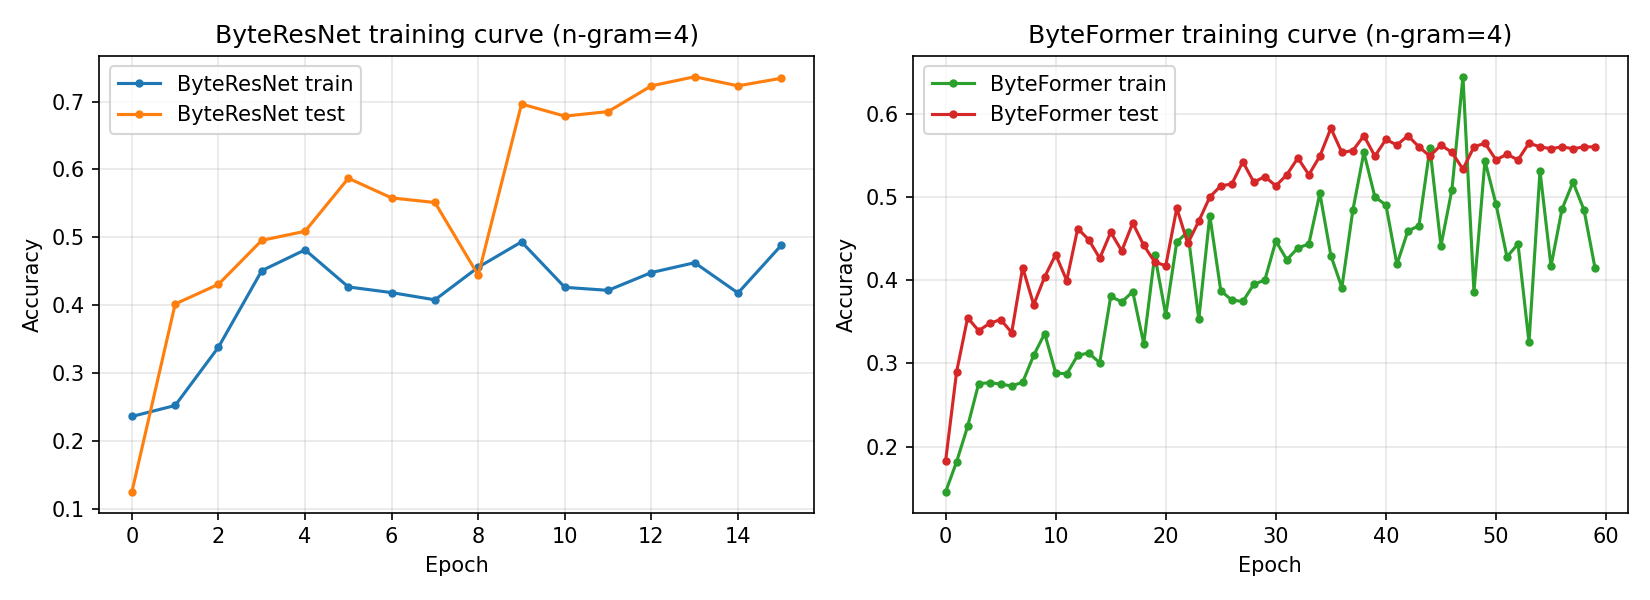
\includegraphics[width=0.95\linewidth]{figures/training_curves.png}
\end{center}
{\footnotesize Train accuracy sits below test accuracy for a mundane
reason: it's computed on mixup-blended batches against soft labels, so
it's noisier by construction, not because the model is struggling.
ByteFormer, on the right, needed almost four times the epochs just to
get into the same neighborhood, and still didn't fully catch up.}
\end{frame}

% ------------------------------------------------------
\begin{frame}{Confusion Matrix -- Where Errors Happen}
\begin{center}
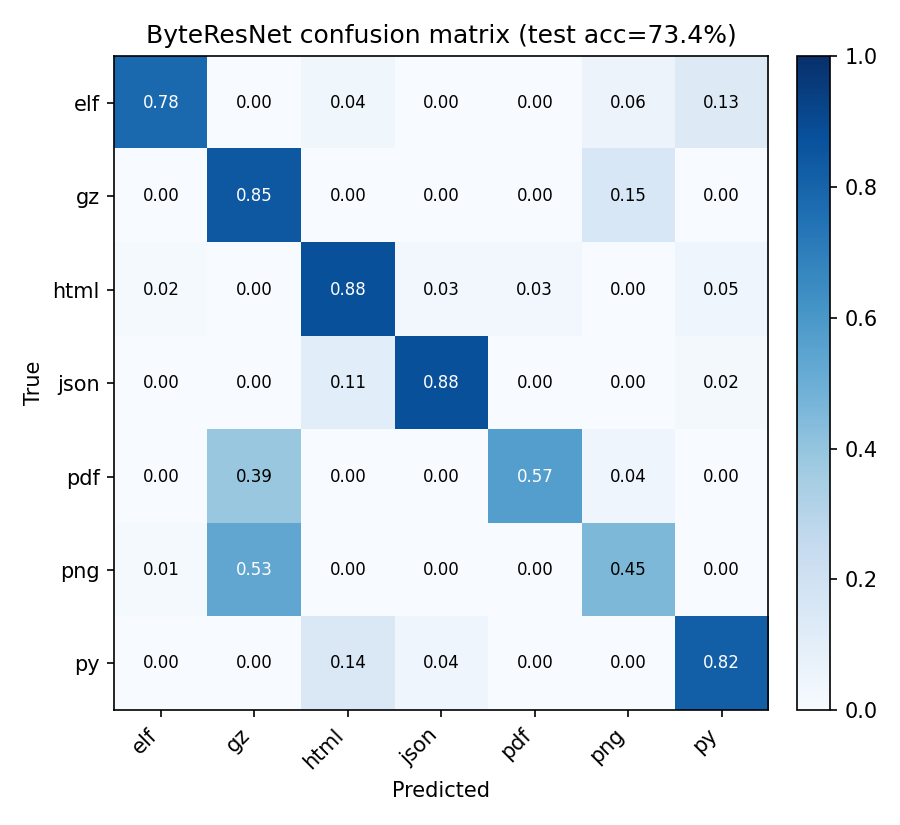
\includegraphics[width=0.5\linewidth]{figures/confusion_matrix.png}
\end{center}
\small
\texttt{pdf}, \texttt{png}, and \texttt{gz} keep getting mixed up with
each other, and there's a real reason for it: PDF embeds
zlib-compressed streams internally, and PNG uses zlib for its own
compression -- at the byte level, compressed data from different
containers just looks similar. The original paper runs into the same
wall between its Archive and Published categories (their Fig.~7).
\end{frame}

% ------------------------------------------------------
\begin{frame}{Branch Ablation}
\begin{center}
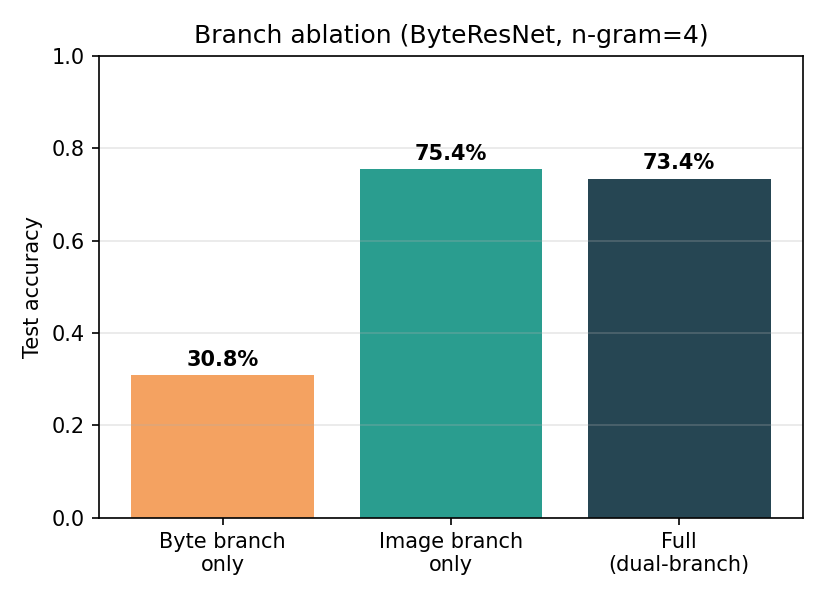
\includegraphics[width=0.62\linewidth]{figures/ablation_branches.png}
\end{center}
Take the image branch away and accuracy drops to 30.8\% -- barely above
guessing. Take the byte branch away instead and it actually goes up
slightly, to 75.4\%. It's the same pattern the paper reports in its
Table~V: the image branch carries almost the entire result, and the byte
branch adds a smaller signal on top of it.
\end{frame}

% ------------------------------------------------------
\begin{frame}{N-gram Sweep \& Variant Comparison}
\begin{columns}
\column{0.5\textwidth}
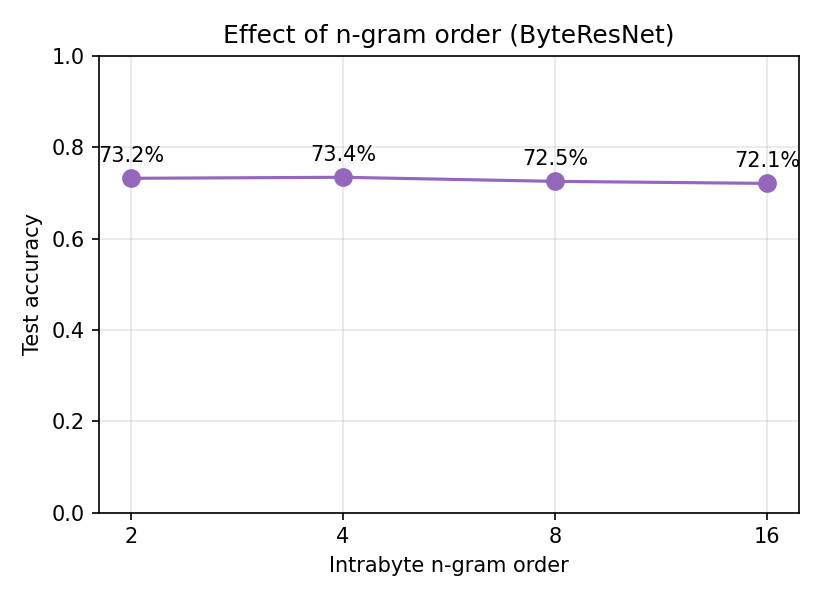
\includegraphics[width=\linewidth]{figures/ngram_sweep.png}
\column{0.5\textwidth}
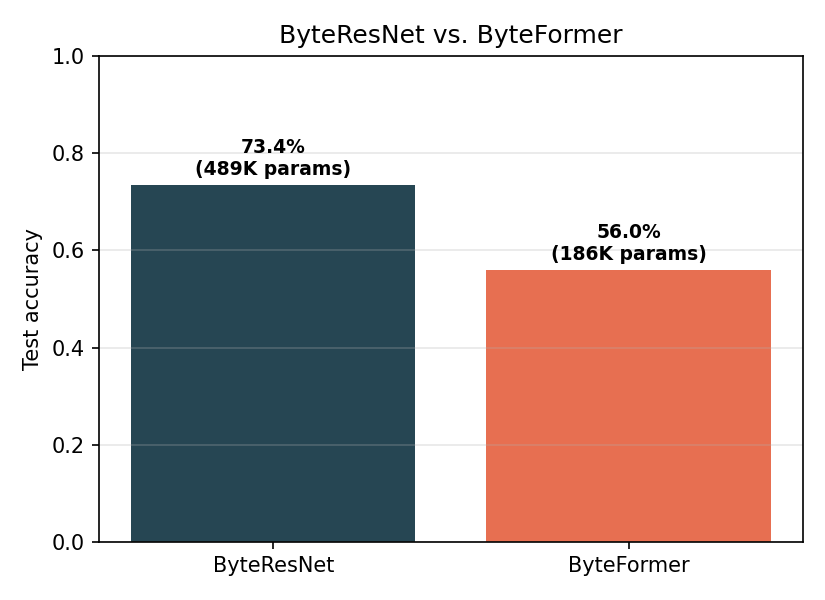
\includegraphics[width=\linewidth]{figures/variant_comparison.png}
\end{columns}
\vspace{0.4em}
\small
On the left: moving the n-gram order from 2 up to 16 only shifts
accuracy by about a point, which lines up with the paper calling
ByteResNet fairly insensitive to this setting.\\
On the right: ByteFormer trains roughly 15$\times$ faster per epoch, but
even at 60 epochs against ByteResNet's 16, it settles well below it.
\end{frame}

% ------------------------------------------------------
\begin{frame}{Honest Discussion: Where We Diverge}
A few places our numbers don't line up with the paper, laid out plainly
rather than buried:
\begin{itemize}
    \item the image-only ablation (75.4\%) edges out the full model
    (73.4\%) -- in the paper, full always wins. Our best guess is that
    the byte branch needs FFT-75-scale data, on the order of 100K
    fragments per class, before it actually pulls its weight. We're
    running 320.
    \item ByteFormer falls further behind here than it does in the
    paper, even with nearly four times the epoch budget -- patch-based
    tokenization probably just needs more data than 2{,}240 fragments
    can give it.
    \item none of these numbers are directly comparable to FFT-75 or
    VFF-16 results anyway -- this is a different, much smaller dataset.
\end{itemize}
\vspace{0.4em}
What ties all three together is scale, not a bug in the implementation
-- everything we could actually test at this size came out the way the
paper says it should.
\end{frame}

% ------------------------------------------------------
\begin{frame}{Our Contribution -- What We Implemented}
None of this is adapted from the authors' repository. Everything below
is code we wrote and ran ourselves:
\begin{itemize}
    \item \texttt{bytenet/byte2image.py} -- the bit-shift and n-gram
    transform, unit-tested on its own before it touched the rest of the
    pipeline
    \item \texttt{bytenet/models.py} -- the byte branch, both embedding
    layers (n-gram and patch), both block types (ResNet and PoolFormer),
    the four-stage backbone, and the fusion step
    \item \texttt{bytenet/data\_prep.py} -- the real 7-class dataset
    builder
    \item \texttt{bytenet/train.py} -- the AdamW plus cosine schedule
    plus mixup training loop, with byte-only and image-only ablation
    modes built in
    \item \texttt{scripts/} -- the experiment runner and figure
    generator that produced every chart in this talk
\end{itemize}
\end{frame}

% ------------------------------------------------------
\begin{frame}{Thank You}
\centering
Code: \texttt{github.com/\textless your-username\textgreater/bytenet-implementation}

\vspace{1em}
Every figure, log, and number in this talk came out of that repository --
nothing here is mocked up.

\vspace{1.5em}
Questions?
\end{frame}

\end{document}
